%    JJJ    AA     CCCCCC KKK   K TTTTTT HH  HH EEEEEE BBBBBB UU  UU SSSSSS    CCCCCC OOOOOO MM  MM
%    JJJ   AAAA    CCCCCC KKK  K  TTTTTT HH  HH EEEEEE BB   B UU  UU SSS       CCCCCC OOOOOO MM  MM
%    JJJ  AA  AA   CC     KKK K     TT   HHHHHH EEE    BB   B UU  UU SSS       CC     OO  OO MMMMMM
%    JJJ AA    AA  CC     KKKK      TT   HHHHHH EEEEEE BBBBBB UU  UU  SSSSS    CC     OO  OO M MM M
%    JJJ AAAAAAAA  CC     KKK K     TT   HH  HH EEE    BB   B UU  UU    SSS    CC     OO  OO M MM M
% JJJJJJ AA    AA  CCCCCC KKK  K    TT   HH  HH EEEEEE BB   B UUUUUU    SSS .. CCCCCC OOOOOO M MM M
% JJJJJJ AA    AA  CCCCCC KKK   K   TT   HH  HH EEEEEE BBBBBB UUUUUU SSSSSS .. CCCCCC OOOOOO M MM M
% 
% Texte Geschrieben von Stefan Bopp und Chantal Frunz
% Mehr Informationen sind auf jackthebus.com zu finden

\subsection{05.05.2016 Ankunft im Welschland}

\begin{wrapfigure}{R}{0.45\textwidth} 
  \begin{centering}
    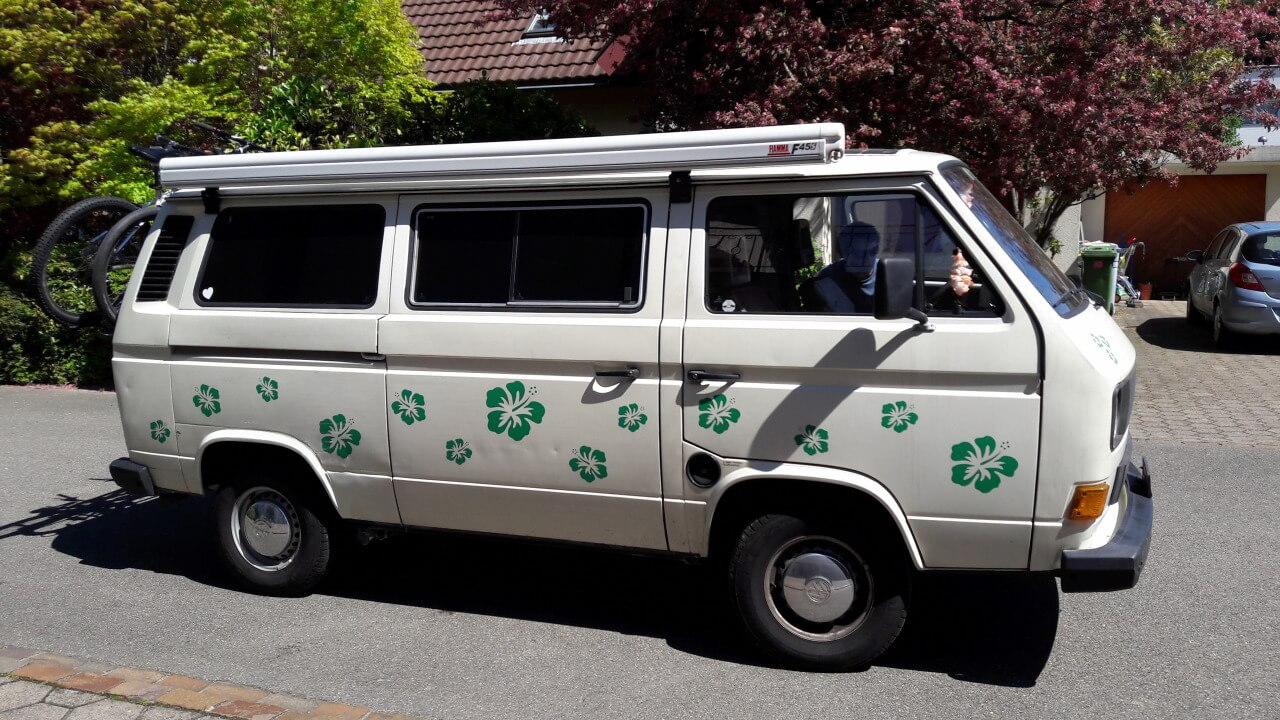
\includegraphics[width=0.4\textwidth, height=5cm, keepaspectratio]{../Bilder/Gruyere/1.jpg}
    \caption{Abfahrt}
  \end{centering}
\end{wrapfigure} 


Zuerst musste Gepäck Fahrräder Personen und der Bus zusammen gebracht werden.
Alles von Luzern nach Nussbaumen, wo der Bus auf uns wartete.
Einmal alles umladen und los ging die Fahrt in das für uns unbekannte Welschland.
So unbekannt war die Region für mich jedoch nicht.
Durfte ich doch 21 Wochen bezahlt von Vater Staat in der Region Payerne verbringen.
Diese Aufenthalte fördern den Ruf einer Gegend normalerweise nicht sonderlich.
Zusätzlich wird gemunkelt, dass in der Region eine sehr komplizierte Sprache gesprochen wird.
Dieser Sprache mächtig zu werden bedarf einiges an Magie, einer gesunden Portion Verrücktheit und sonst eines am Löffel.

Nach kurzem Stau auf der Autobahn zeigten sich die Berner Alpen am Horizont bei wunderbarer Fernsicht.
Der Campingplatz würde Dank modernster Navigationsmittel problemlos gefunden und die Reihe vor der Rezeption glich einer Bus-Parade.
Der Versprochene Platz direkt am See war dann auch Wirklichkeit (Dank Reservation) und ein kleines Restaurant direkt am Campingplatz sollte uns mit Speisen und Trank versorgen können.

\begin{wrapfigure}{L}{0.45\textwidth} 
  \begin{centering}
    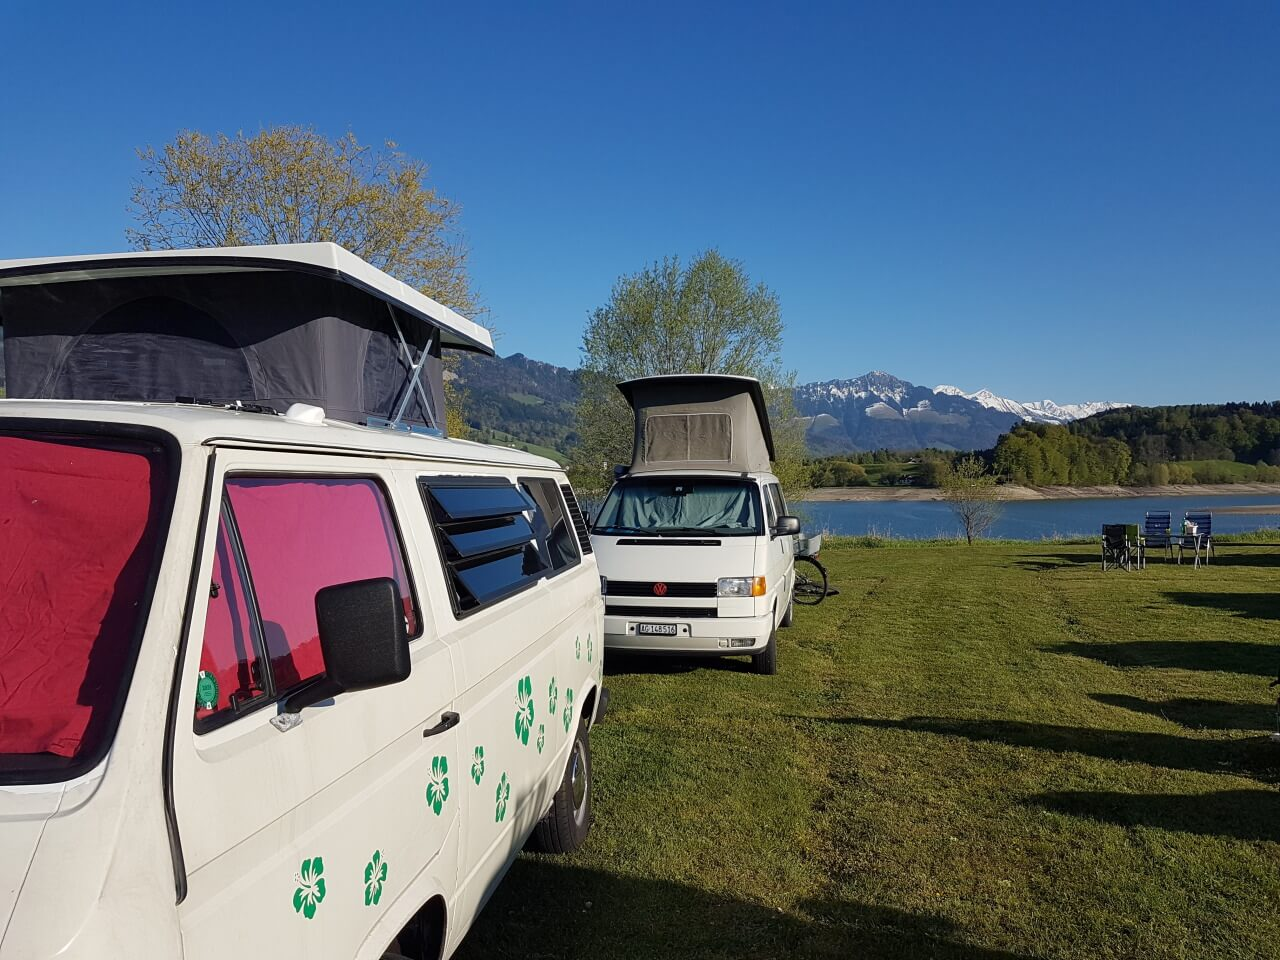
\includegraphics[width=0.4\textwidth, height=5cm, keepaspectratio]{../Bilder/Gruyere/5.jpg}
    \caption{Einreihen}
  \end{centering}
\end{wrapfigure} 

Nach dem Aufstellen und einem kurzen Spaziergang am See, welcher ich zur Zeit vor allem mit einem sehr tiefen Wasserstand bemerkbar macht, kam die Einsicht, dass das ganze mit dem Strom für unseren Ofen eine eher schwierige Angelegenheit wird.
Die Standplätze selbst waren nicht mit einer eigenen Stromversorgung ausgerüstet, sondern es stand ein Bau-Provisorium in einer Ecke.
Der Rest der Verteilung des Stromes war dann dem Zufall überlassen.
Gerade die kalte Nacht, welche auf uns wartete, erhöhte die Wahrscheinlichkeit des Scheiterns des Systems erheblich.
Sowieso waren leider die Plätze am See noch gar nicht erschlossen.
So wurde entschieden die Nacht ohne Ofen zu verbringen.
Sind ja nicht aus Zucker.
Das Restaurant trumpfe gross auf.
Mit einem 300 gr. Steak auf dem heißen Stein und Wein im Überfluss machte es bei mir sehr viele Punkte gut.
Nach einem Test des neuen Multimediasystem des Buses hieß es sich warm einzupacken und seit langer Zeit wieder einmal im Bus zu schlafen.

\begin{figure}[hb]
    \centering
    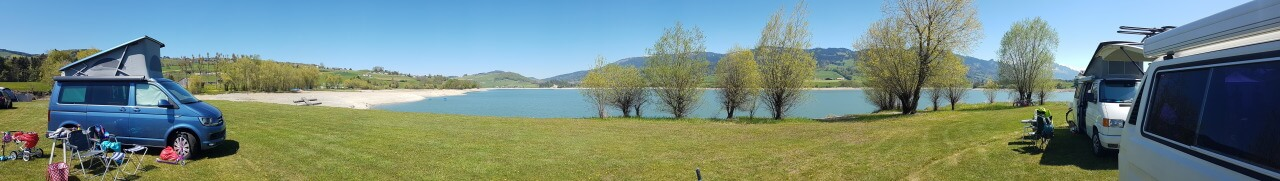
\includegraphics[width=\textwidth]{../Bilder/Gruyere/3.jpg}
    \caption{Platz am See}
    \label{img:Gruyere}
\end{figure}

\subsection{06.05.2016 Stürmt das Schloss Gruy\`{e}res}

\begin{wrapfigure}{L}{0.45\textwidth} 
  \begin{centering}
    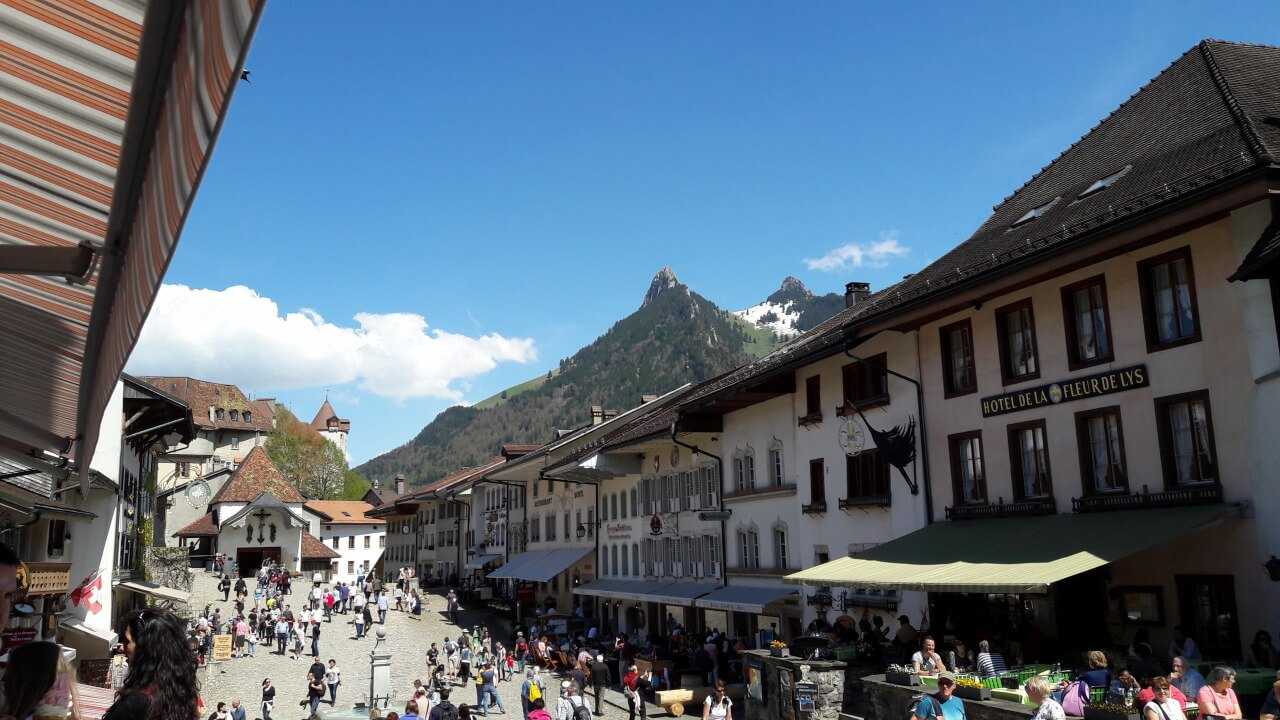
\includegraphics[width=0.4\textwidth, height=5cm, keepaspectratio]{../Bilder/Gruyere/10.jpg}
    \caption{Gruyere}
  \end{centering}
\end{wrapfigure} 

Oh ja, Herstellerangaben sollte man glauben.
Der Comfort-Bereich meines Schlafsack ist bei warmen 13°C nach unten beschränkt.
Die klare Nacht hielt nichts von diesem Limit und näherte sich erbarmungslos der 0° Grenze.
Gegen Null ging auch die Laune von Chantal nach dem ich sie unter einer Unmenge von Decke am Morgen nach ihrem Befinden fragte.
Ne, eine weiter Nacht ohne wärmenden Ofen kommt nicht in Frage.
So konnte die Frage nach Strom ganz zu oberst auf der Prioritätenliste gefunden werden.
Nach mehrmaligen hin und her fanden wir dann auch einen freien Steckplatz in dem nach asiatischen Vorbild natürlich gewachsenen Stromnetz.
Die Warnung, dass an diesem Knoten bereits 3 Ofen angeschlossen seien, stimmte nicht gerade zuversichtlich.
Man wird sehen.
Nach einem reichhaltigen Frühstück direkt am See wurden Pläne für eine Velotour geschmiedet.
Rucksäcke gepackt Google Maps nach der Route befragt und los kann es gehen.

Die anfängliche Route der Hauptstraße entlang könnte nicht begeistern und so wurde schon bald ein Abzweiger gefunden, welcher uns die typische Gegend näher bringen sollte.
Nicht gerade Zielgerichtet ging es voran, aber immerhin schön ruhig und sehenswert.
Pools scheine hier niemanden zu Interessieren.
Dafür Trampolins.
Jeder der was auf sich hält hat so ein Ungetüm im Garten.
Beim ersten Abchecken der Karte wurde ein Bewohner sofort auf uns aufmerksam und fragte nach ob alles in Ordnung sei.
Überall sehr nette Menschen.
So ging es weiter mit einer Zusatzschlaufe zum Chocolatier Cailler.
Schon bald war die Sicht frei auf das Schloss Gruy\`{e}res.
Nur noch ein Flugplatz war im Weg.
Der wurde prompt für eine Zwischenverpflegung genutzt.
Ein Fehler.
Nach diesem Stop war es vorbei mit Velotour.
Nun begann die Velotortur.
Der Plan Gruy\`{e}res per Velo zu befahren würde schnell zerschlagen und wir beschlossen das Vorhaben per Pedes abzuschliessen.
Eine Unmenge Touristen bevölkerten das kleine Dörfchen.

\begin{figure}[H]
   \centering
      %\subfloat[CAPTION]{BILDERCODE}\qquad
   \subfloat{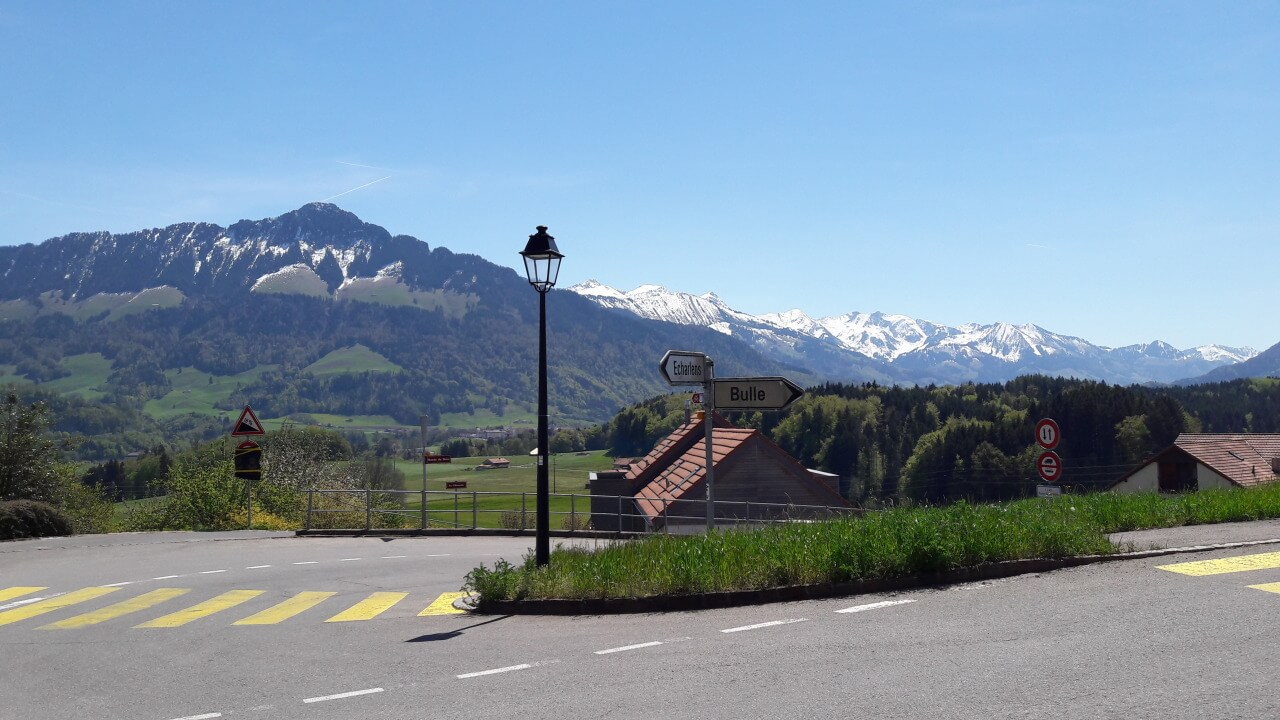
\includegraphics [width=0.3\textwidth]{../Bilder/Gruyere/8.jpg}}\quad
   \subfloat{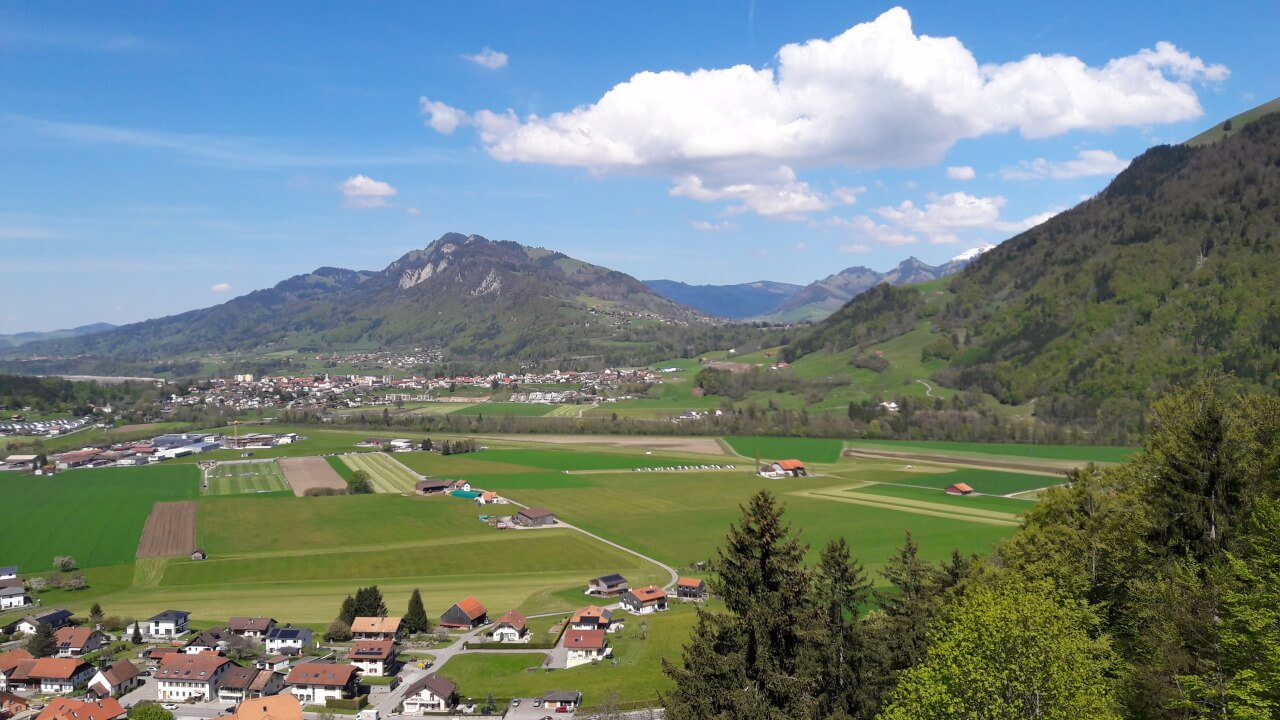
\includegraphics [width=0.3\textwidth]{../Bilder/Gruyere/11.jpg}}\quad
   \subfloat{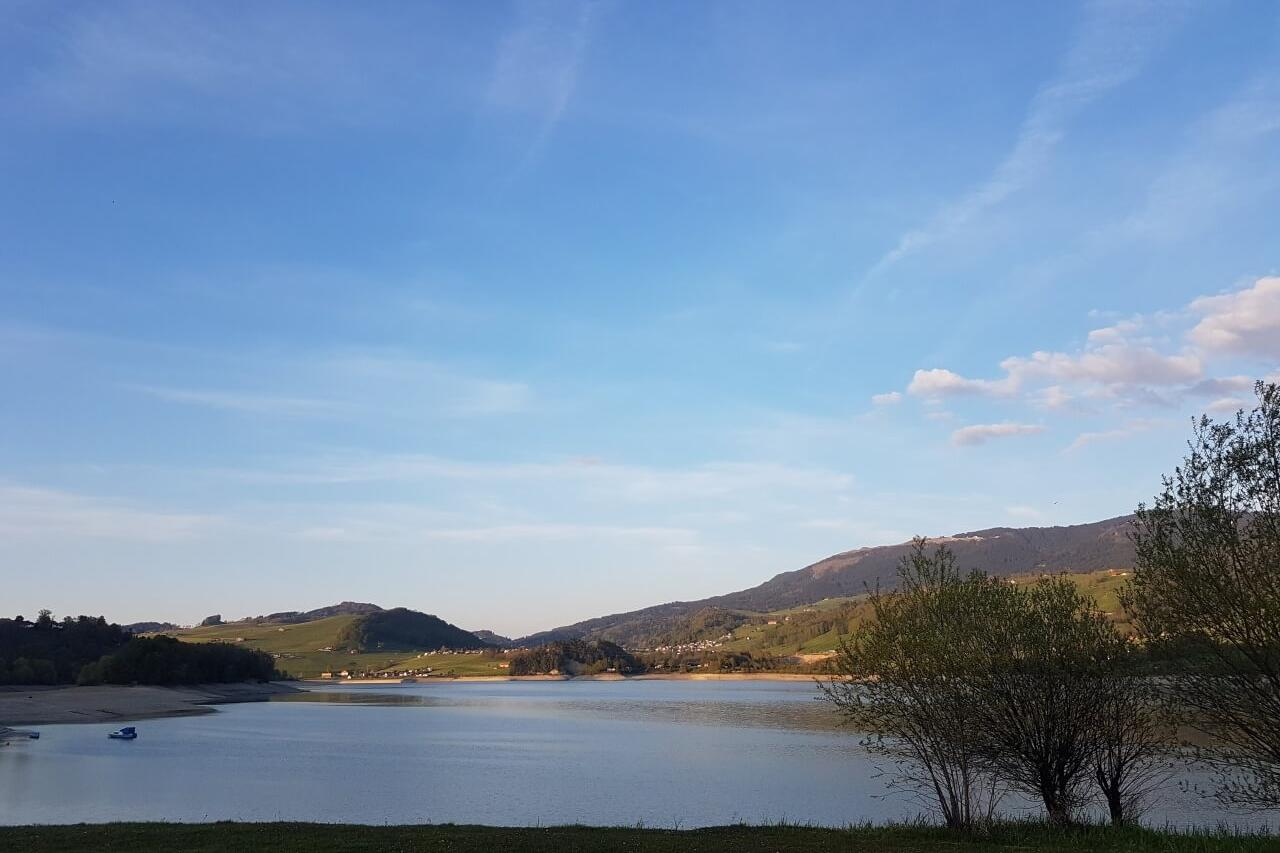
\includegraphics [width=0.3\textwidth]{../Bilder/Gruyere/12.jpg}}\quad
   \caption[Impressionen von der Velotour]{Impressionen von der Velotour}
\end{figure}

Nach einer kurzen Stärkung und Besichtigung des Rummels war es an der Zeit die Müden Beine (von was eigentlich??) wieder auf dem Velo abzustrampeln.
Bulle war das Ziel.
20 Min später wurde Bulle erkundet und nach etwas Nahrhaftem abgesucht.
Crepes wurden ausgesucht, da die doch eher frühe Stunde der Auswahl nicht gerade dienlich war.
Das letzte Teilstück ging dann überraschend flott von statten.
Bald könnte die Dusche genossen werden.
Naja, sofern man 50 Räppler dabei hatte.
Sonst hiess eher kalt zu duschen.
Chantal kann da ein Lied von singen.
Nach einem kurzen Kochversuch im Bus (Suppe und Tee) schlüpften wir in die Schlafsäcke und harrten der Dinge die da kommen.
Der Ofen funktionierte die ersten 10 Minuten problemlos.
Dann war jedoch für andere auch Schlafenszeit und die Sicherung wurde überbeansprucht.
Doch irgendeine gute Seele gab ihr eine zweite Chance und hat sie wieder rein gemacht.
Dies verhinderte eine weitere kalte Nacht.

\subsection{07.05.2016 Creux du Van}

\begin{wrapfigure}{L}{0.45\textwidth} 
  \begin{centering}
    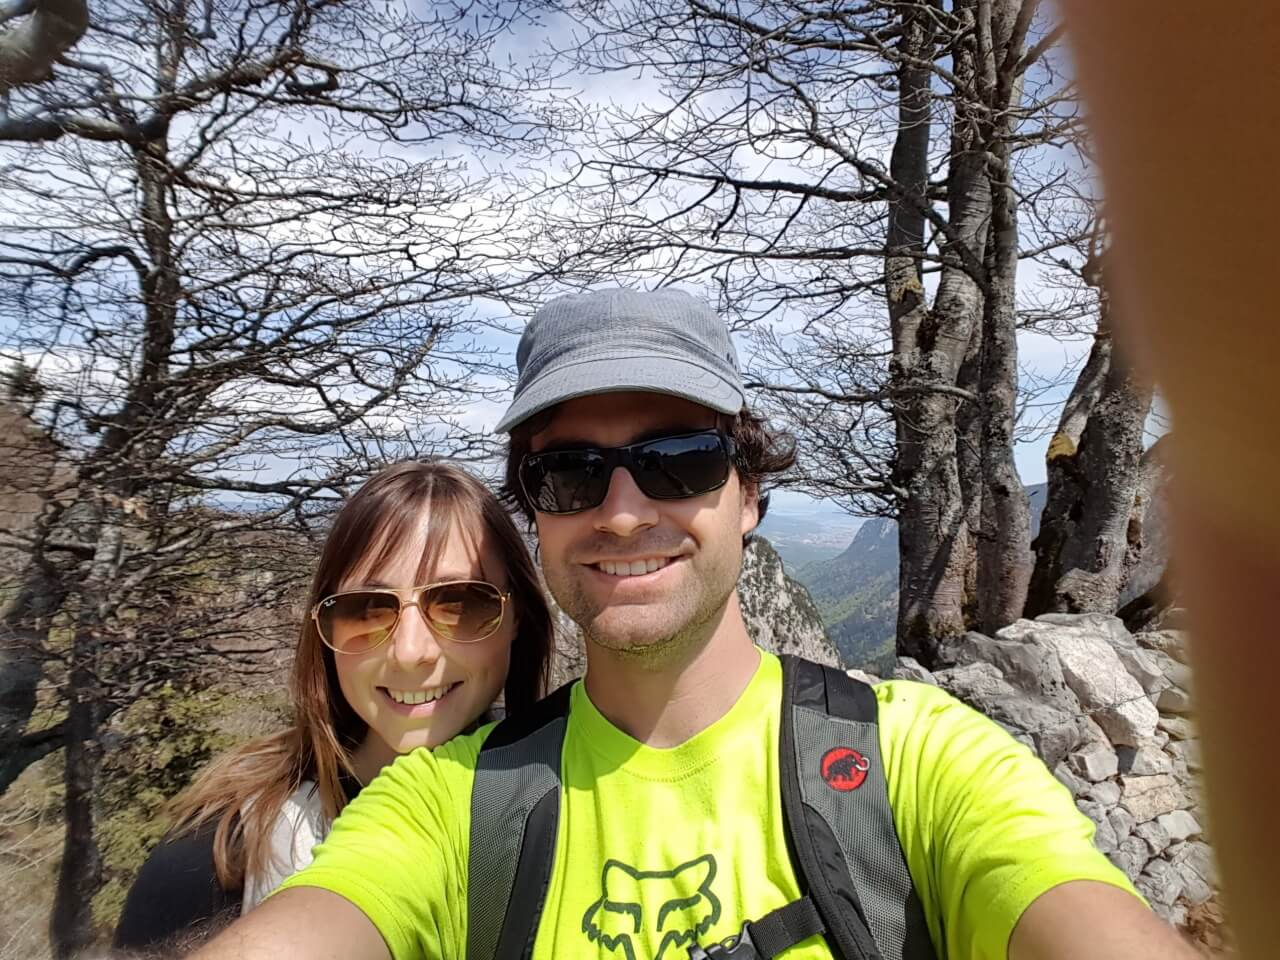
\includegraphics[width=0.4\textwidth, height=5cm, keepaspectratio]{../Bilder/Gruyere/17.jpg}
    \caption{Selfie vor der bekannten Wand}
  \end{centering}
\end{wrapfigure} 

Heute hiess es: Fahrt an den Neuenburger-See und Wanderung auf den Creux du Van.
Nach einer erholsamen Nacht (schön warm).
Wurde das nötigste Zusammengepackt und die anderen Campingbewohner mit einer schönen Rauchwolke zu ihrem Morgenessen begrüsst.
Los ging es.
Kreuz und Quer ging es durch das Welschland und das bei schönstem Wetter.
Dank Kollege Google fanden wir auch das kleine Dörfchen Noiraigue, der Ausgangspunkt unserer Wanderung.
Kurz vor dem Ankommen mussten noch die Spritvorräte sowie die Verpflegung aufgefrischt werden.
Saucisse à l'ail fand den Weg in den Einkaufskorb.
Mit etwas Glück konnten wir einen der letzten Parkplätze erhaschen.
Ab in die Wanderschuhe und los Richtung Bahnhof.
Den Weg kann man jetzt wirklich nicht verfehlen.
Etliche Personen hatten den gleichen Plan.
Ungefähr nach der Hälfte des Aufstiegs befindet sich ein Hof, welcher Leckereien verkauft.

Diese Chance musste natürlich gepackt werden.
Nach zweieinhalb Stunden Aufstieg erreichten wir die Krete und konnten ein erstes Mal die imposante Wand bestaunen.
Das einzig unschöne: 300 Meter vom Abriss entfernt war ein Restaurant, welches mit dem Auto erreichbar ist.
Dementsprechend viele Besucher lockte dieser Ort, welcher noch leicht erreichbar ist an.

Nach einem Picknick und der Erkenntnis, dass die Tagesform einen riesigen Unterschied macht, ging es noch bis zum Punkt le Soliat.
Von dort hiess es die vorher gemachten 700 Höhenmeter in Muskelkater umzuwandeln.
Immer runter ging es bis wir nach 1 3/4 Stunden zufrieden und eigentlich noch ganz fit wieder ankamen.
Nur Chantals Beine wollten das ewige Bremsen nicht so recht gefallen und so musste ein Stock als Hilfe beschafft werden.

\begin{figure}[h]
   \centering
      %\subfloat[CAPTION]{BILDERCODE}\qquad
   \subfloat{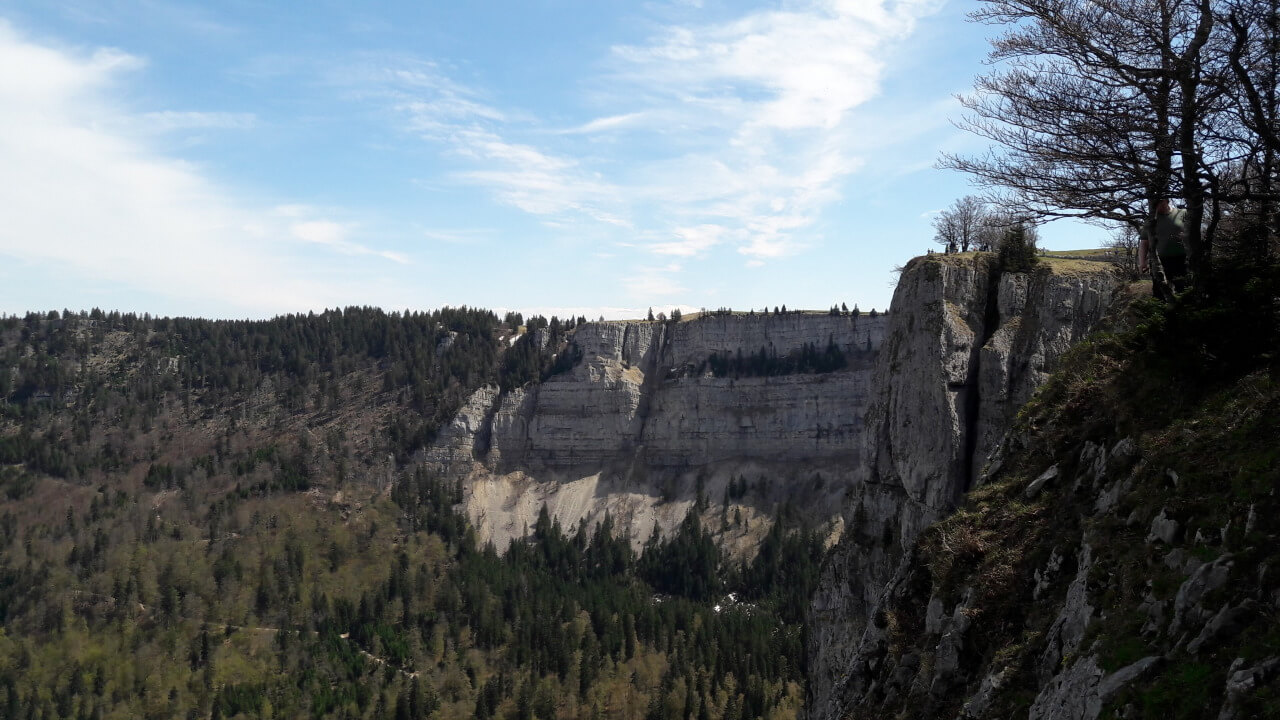
\includegraphics [width=0.3\textwidth]{../Bilder/Gruyere/19.jpg}}\quad
   \subfloat{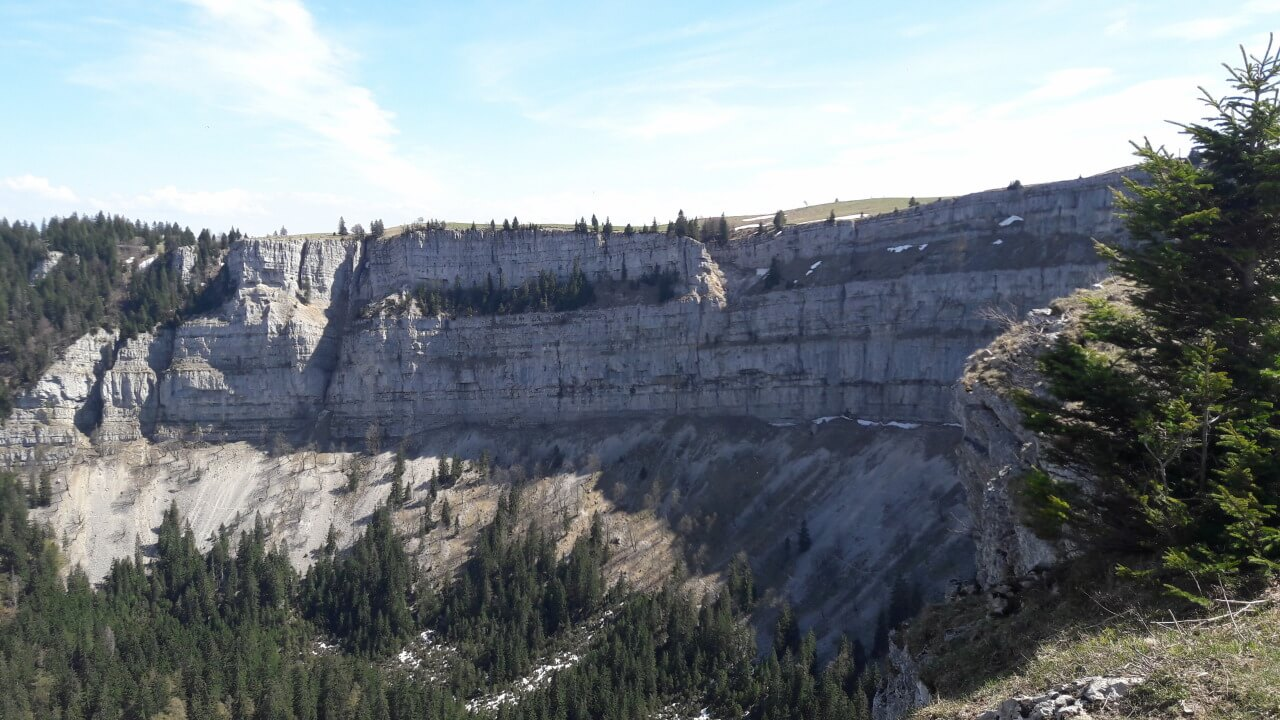
\includegraphics [width=0.3\textwidth]{../Bilder/Gruyere/20.jpg}}\quad
   \subfloat{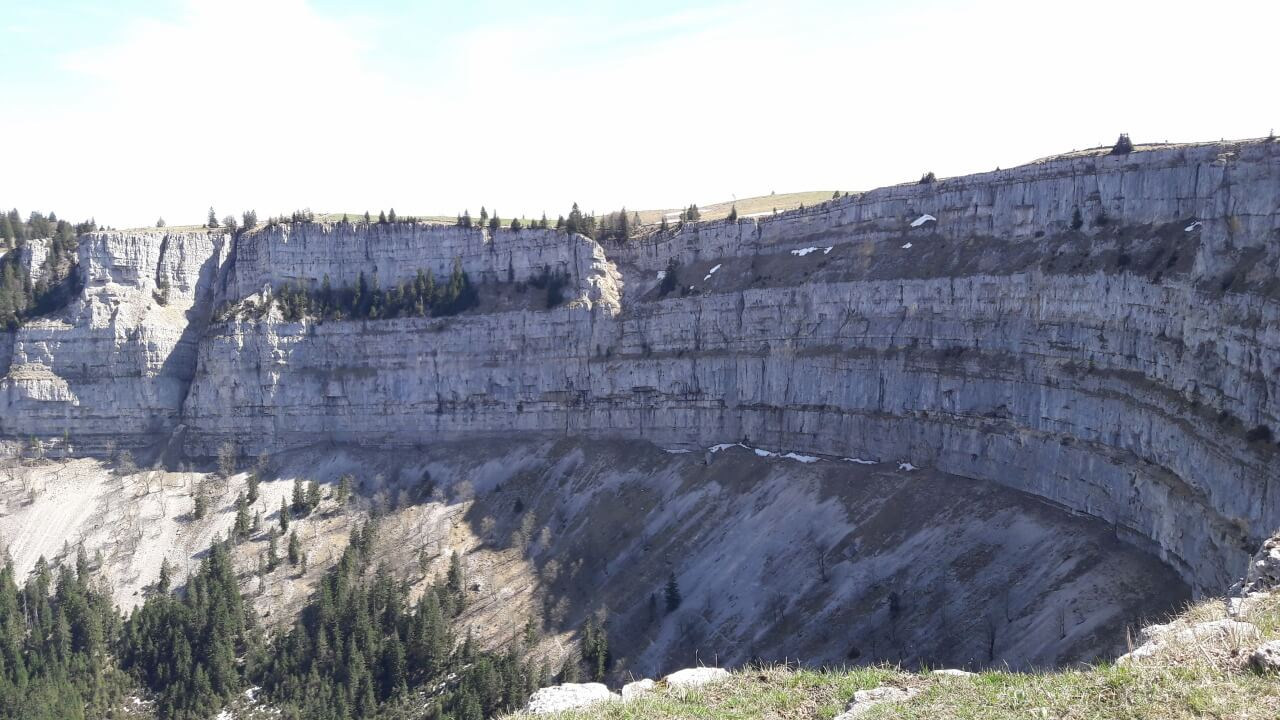
\includegraphics [width=0.3\textwidth]{../Bilder/Gruyere/21.jpg}}\quad
   \caption[Creux du van]{Creux du van}
\end{figure}

Wie schon das ganze Weekend waren auch hier wieder unzählige VW Busse unterwegs.
Die Fahrt zurück wurde nur durch eine extensive Anordnung von unnötigen Kreiseln unterbrochen.
Teilweise reichte der Platz zwischen zwei Kreisel nicht einmal für ein Stück Strasse.
So wuchsen zwei Kreisel zusammen.
Da wir eh an dem Camping-Restaurant vorbei mussten, war es nahe liegend gleich noch da zu reservieren.
Nach der Dusche und einem feinen Essen Fischknüsperli (wie man hier zu sagen pflegt) ginge es für eine weitere (leider die letzte Nacht im VW Bus, in dem uns die Heizung glücklicherweise nicht im Stich lies.

\begin{figure}[hb]
    \centering
    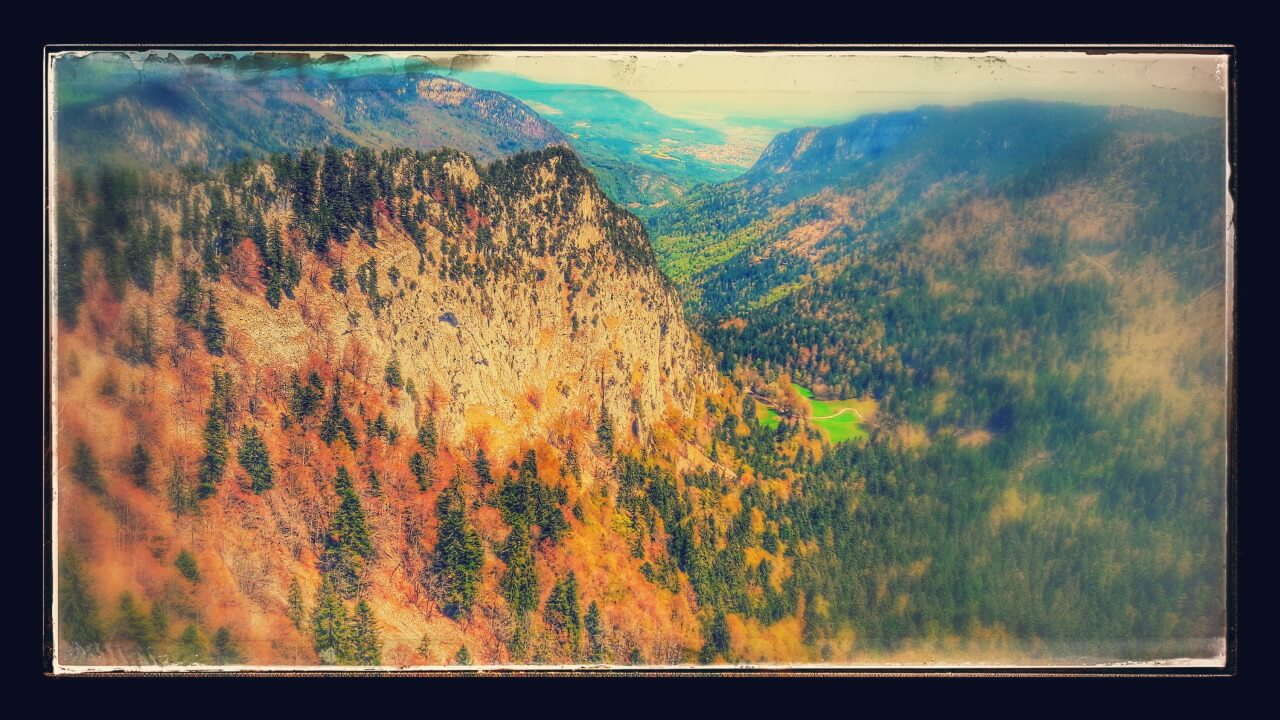
\includegraphics[width=\textwidth]{../Bilder/Gruyere/18.jpg}
    \caption{Creux du van}
    \label{img:Gruyere2}
\end{figure}

\subsection{08.05.2016 Retour und Fribourg}

\begin{wrapfigure}{L}{0.45\textwidth} 
  \begin{centering}
    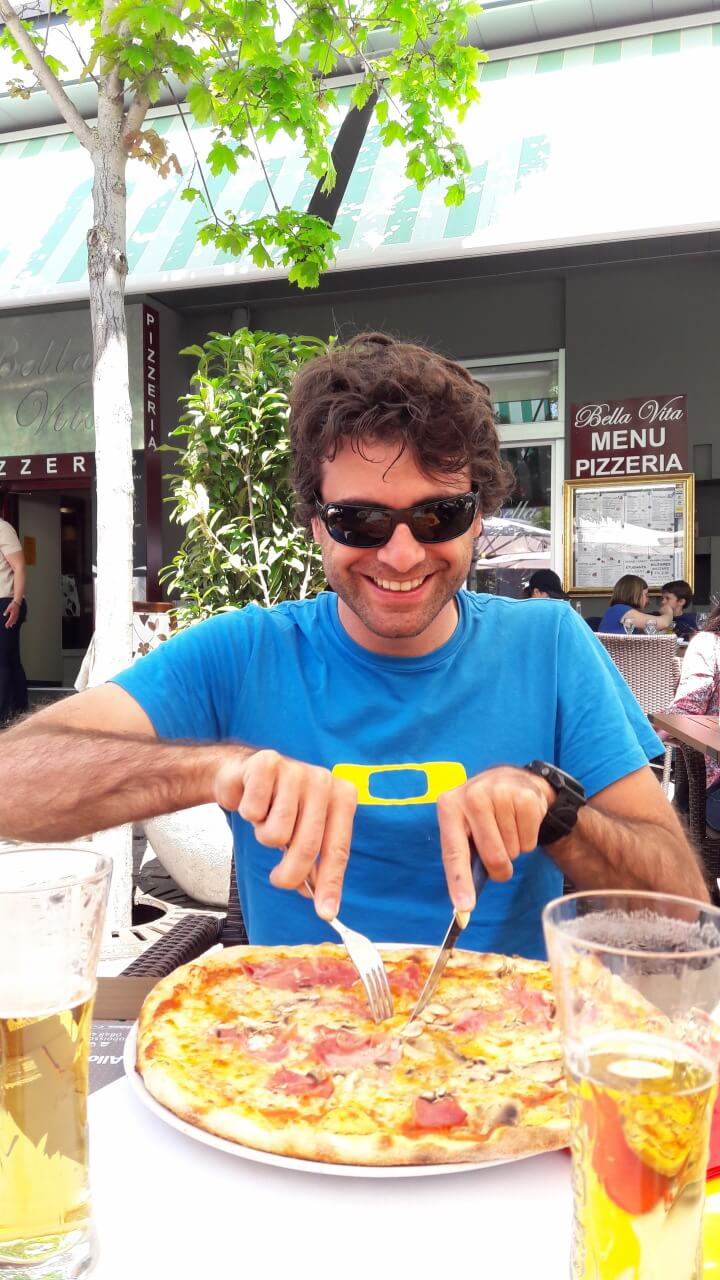
\includegraphics[width=0.4\textwidth, height=5cm, keepaspectratio]{../Bilder/Gruyere/26.jpg}
    \caption{PIZZAAAAA}
  \end{centering}
\end{wrapfigure} 

Chantal war schon früh auf den Beinen und bevor ich mich überhaupt das erste Mal bewegte stand das Frühstück schon bereit.
Es brach richtiggehend Hektik aus und der ganze Campingplatz schien sich auf den Weg zu machen.
Überall wurde Gepackt, verstaut und losgefahren.
Auch wir setzten uns um 11 in den Bus und machten uns auf den Weg Richtung Fribourg.
Ein Parkplatz war schnell gefunden und das angenehme Wetter lud zu einer kleinen Stadtbesichtigung ein.
Die bessere Hälfte fand sich vor einer Unmenge an interessanten Geschäften, welche zum Glück eines gemeinsam hatten: Sie waren geschlossen.
Eine Pizzeria zog mich magisch in den Bann und schon bald sassen wir das und genossen ein Mittagessen an der Sonne.

Der Rückweg über die Autobahn war dann ereignislos.
Schon bald konnten wir das ganze Spiel mit Gepäck, Essen und Velos verladen ein weiteres mal machen und den Bus wieder auf den bekannten und geschätzten Parkplatz stellen.
Nach vier kurzen Tagen im Welschland bleibt folgendes zu sagen:

Resümee (das Wort gibt es tatsächlich so) 

\begin{itemize}
    \item Knoblauchwurst, Brot und Bier in Kombination schlägt alles Doping der Welt.

    \item Der Mond ist am Lac de Gruyere nicht sichtbar (fragt Chantal für Details)

    \item Französisch zu sprechen ist und bleibt mühsam

    \item Trotzdem lohnt sich der Besuch auf der anderen Seite des Röstigrabens auf jeden Fall

    \item Chantal würde auch als Gandalf eine gute Figur machen

    \item Multimediasystem im Bus,  Schön und gut aber unnütz.

    \item Neues Dach dafür leider geil

    \item Fribourg auf jeden Fall wieder einmal ein Besuch wert!
\end{itemize}
